\begin{center}
	\textbf{ÔN TẬP KIỂM TRA HỌC KÌ 2}\\
	\textbf{ NĂM HỌC 2024 -2025}
%	\textbf{CHƯƠNG 6: NĂNG LƯỢNG}
\end{center}
\Opensolutionfile{ans}[ans/ONTAPHK2-TL]

% ===============================================================
\begin{ex}
	Một vận động viên nhảy dù có khối lượng \SI{70}{\kilogram} thực hiện động tác nhảy dù từ độ cao \SI{500}{\meter} so với mặt đất. Sau một đoạn đường rơi tự do thì vận động viên bật dù và tiếp đất với vận tốc \SI{8}{\meter/\second}. Lấy $g=\SI{9.8}{\meter/\second^2}$.
	\begin{enumerate}[label=\alph*)]
		\item Tính thế năng của vận động viên so với mặt đất trước khi nhảy dù.
		\item Tính động năng của vận động viên khi tiếp đất.
		\item Tính công của lực cản của không khí.
	\end{enumerate}
	\loigiai{
		
	}
\end{ex}
% ===============================================================
\begin{ex}
	Một tàu lượn siêu tốc có điểm cao nhất cách điểm thấp nhất \SI{94.5}{\meter} theo phương thẳng đứng. Tàu lượn được thả không vận tốc ban đầu từ điểm cao nhất. Lấy $g=\SI{9.8}{\meter/\second^2}$.
	\begin{enumerate}[label=\alph*)]
		\item Tìm vận tốc cực đại mà tàu lượn có thể đạt được.
		\item Trên thực tế, vận tốc cực đại của tàu lượn đạt được là \SI{41.1}{\meter/\second}. Tính hiệu suất của quá trình chuyển đổi thế năng thành động năng của tàu lượn.
	\end{enumerate}
	\loigiai{
		
	}
\end{ex}
% ===============================================================
\begin{ex}
	Một ô tô có khối lượng 4 tấn đang chuyển động với vận tốc \SI{72}{\kilo\meter/\hour} trên một đoạn đường nằm ngang thì hãm phanh. Sau khi đi được quãng đường \SI{50}{\meter} thì vận tốc của ô tô giảm xuống còn \SI{36}{\kilo\meter/\hour}.
	\begin{enumerate}[label=\alph*)]
		\item Tính lực hãm trung bình của ô tô.
		\item  Nếu vẫn giữ nguyên lực hãm trung bình đó thì kể từ lúc hãm phanh ô tô đi được quãng đường bao nhiêu rồi dừng lại?
	\end{enumerate}
	\loigiai{
		
	}
\end{ex}
% ===============================================================
\begin{ex}
	Một vật khối lượng \SI{0.5}{\kilogram} được thả rơi từ độ cao \SI{25}{\meter}. Bỏ qua mọi ma sát và lấy $g=\SI{10}{\meter/\second^2}$. Chọn gốc thế năng tại mặt đất.
	\begin{enumerate}[label=\alph*)]
		\item Tính thế năng của vật lúc bắt đầu thả. Suy ra cơ năng của vật.
		\item Tính thế năng của vật ở độ cao \SI{15}{\meter}. Suy ra động năng của vật tại vị trí này.
		\item Tìm độ cao của vật khi nó có động năng bằng thế năng.
		\item Tìm tốc độ của vật tại vị trí có thế năng bằng $\dfrac{1}{3}$ cơ năng.
		\item Tìm tốc độ của vật khi nó có thế năng bằng ba lần động năng.
		\item Tìm tốc độ của vật khi chạm đất.
	\end{enumerate}
	\loigiai{
		
	}
\end{ex}
%\begin{center}
%	\textbf{CHƯƠNG 7: ĐỘNG LƯỢNG VÀ ĐỊNH LUẬT BẢO TOÀN ĐỘNG LƯỢNG}
%\end{center}
%% ===============================================================
%\begin{ex}
%	Một quả bóng golf có khối lượng \SI{46}{\gram} đang nằm yên, sau một cú đánh quả bóng bay lên với tốc độ \SI{70}{\meter/\second}. Tính xung lượng của lực và độ lớn trung bình của lực tác dụng vào quả bóng. Biết thời gian tác là \SI{0.5E-3}{\second}.
%	\loigiai{
%		
%	}
%\end{ex}
% ===============================================================
\begin{ex}
	Một viên đạn có khối lượng $m = \SI{10}{\gram}$ đang bay với vận tốc $v_1=\SI{1000}{\meter/\second}$  thì gặp bức tường. Sau khi xuyên qua bức tường thì vận tốc của viên đạn còn lại là $v_2=\SI{400}{\meter/\second}$. Tính độ biến thiên động lượng và lực cản trung bình của bức tường lên viên đạn? Biết thời gian xuyên thủng tường là \SI{0.01}{\second}.
	\loigiai{
		
	}
\end{ex}
% ===============================================================
\begin{ex}
	Một quả lựu đạn đang bay theo phương ngang với vận tốc \SI{10}{\meter/\second} thì bị nổ và tách thành hai mảnh có trọng lượng \SI{10}{\newton} và \SI{15}{\newton}. Sau khi nổ, mảnh to vẫn chuyển động theo phương ngang với vận tốc \SI{25}{\meter/\second} cùng chiều chuyển động ban đầu. Lấy $g\approx\SI{10}{\meter/\second^2}$. Xác định vận tốc và phương chuyển động của mảnh nhỏ.
	\loigiai{
		
	}
\end{ex}
%% ===============================================================
%\begin{ex}
%	Quả cầu thứ nhất có khối lượng \SI{2}{\kilogram} chuyển động với vận tốc \SI{3}{\meter/\second}, tới va chạm vào quả cầu thứ hai có khối lượng \SI{3}{\kilogram} đang chuyển động với vận tốc \SI{1}{\meter/\second} cùng chiều với quả cầu thứ nhất trên một máng thẳng ngang. Sau va chạm, quả cầu thứ nhất chuyển động với vận tốc \SI{0.6}{\meter/\second} theo chiều ban đầu. Bỏ qua lực ma sát và lực cản. Xác định chiều chuyển động và vận tốc của quả cầu thứ hai.
%	\loigiai{
%		
%	}
%\end{ex}
% ===============================================================
\begin{ex}
	Một viên đạn pháo khối lượng $m_1=\SI{10}{\kilogram}$ bay ngang với vận tốc $v_1=\SI{500}{\meter/\second}$ dọc theo đường sắt và cắm vào toa xe chở cát có khối lượng $m_2=\SI{1}{\text{tấn}}$, đang chuyển động với tốc độ $v_2=\SI{36}{\kilo\meter/\hour}$. Xác định vận tốc của toa xe ngay sau khi trúng đạn trong hai trường hợp:
	\begin{enumerate}[label=\alph*)]
		\item Đạn bay đến cùng chiều chuyển động của xe cát.
		\item Đạn bay đến ngược chiều chuyển động của xe cát.
	\end{enumerate}
	\loigiai{
		
	}
\end{ex}
%% ===============================================================
%\begin{ex} 
%	\immini{Một quả cầu nhỏ khối lượng $m_1=\SI{200}{\gram}$ treo vào đầu một sợi dây nhẹ không dãn có chiều dài $\ell=\SI{90}{\centi\meter}$. Kéo quả cầu lệch khỏi vị trí cân bằng để dây treo hợp với phương thẳng đứng một góc \SI{60}{\degree} rồi buông nhẹ. Bỏ qua ma sát và các lực cản. Cho $g=\SI{10}{\meter/\second^2}$. 
%		\begin{enumerate}[label=\alph*)]
%			\item Tìm tốc độ của quả cầu $m_1$ tại vị trí thấp nhất của quỹ đạo.
%			\item Tại vị trí cân bằng, quả cầu $m_1$ va chạm đàn hồi với quả cầu $m_2=\SI{50}{\gram}$ đang đứng yên trên mặt sàn nằm ngang. Tìm vận tốc của mỗi quả cầu ngay sau va chạm.
%		\end{enumerate}
%	}
%	{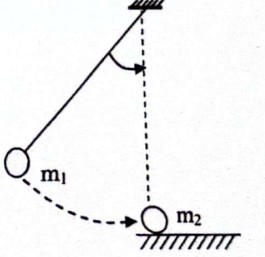
\includegraphics[scale=0.5]{../figs/D10-CK2-001-4}}
%	\loigiai{
%		
%	}
%\end{ex}
%\begin{center}
%	\textbf{CHƯƠNG 8: CHUYỂN ĐỘNG TRÒN}
%\end{center}
% ===============================================================
\begin{ex}
	Một mô tơ điện quay quanh trục với tốc độ \SI{3600}{rpm} (revolutions/min: vòng/phút). Tốc độ góc của mô tơ này bằng bao nhiêu?
	\loigiai{
		
	}
\end{ex}
% ===============================================================
\begin{ex}
	Một chiếc xe chuyển động theo hình vòng cung với tốc độ \SI{36}{\kilo\meter/\hour} và gia tốc hướng tâm \SI{4.0}{\meter/\second^2}. Giả sử xe chuyển động tròn đều. Hãy xác định:
	\begin{enumerate}[label=\alph*)]
		\item bán kính đường vòng cung.
		\item góc quét bởi bán kính quỹ đạo (theo rad và độ) sau thời gian \SI{3}{\second}.
	\end{enumerate}
	\loigiai{
		
	}
\end{ex}
% ===============================================================
\begin{ex}
	So sánh tốc độ góc, tốc độ dài và gia tốc hướng tâm của các đầu kim phút và kim giây trên một đồng hồ. Biết chiều dài kim phút bằng $\dfrac{3}{4}$ chiều dài kim giây.
	\loigiai{
		
	}
\end{ex}
% ===============================================================
\begin{ex}
	Một trái bóng được buộc vào một sợi dây và quay tròn đều trong mặt phẳng nằm ngang như hình bên dưới. Trái bóng quay một vòng trong \SI{1}{\second} với tốc độ \SI{0.5}{\meter/\second}. Tính bán kính quỹ đạo và chiều dài $L$ của sợi dây, biết góc hợp bởi dây và phương thẳng đứng bằng \SI{30}{\degree}.
	\begin{center}
		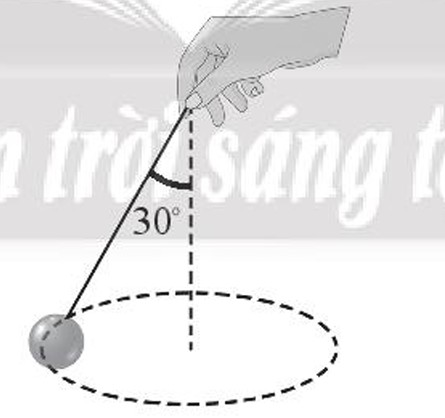
\includegraphics[scale=0.4]{../figs/D10-CK2-003-2}
	\end{center}
	\loigiai{
		
	}
\end{ex}
% ===============================================================
\begin{ex}
	\immini{Cho thanh thẳng AB chiều dài $L = \SI{1.5}{\meter}$ quay đều xung quanh trục đi qua điểm O trên thanh và vuông góc với thanh. Tốc độ của hai đầu thanh lần lượt là $v_{\mathrm{A}}=\SI{2}{\meter/\second}$  và $v_{\mathrm{B}}=\SI{4}{\meter/\second}$. 
		Tính tốc độ góc $\omega$ của thanh và gia tốc hướng tâm tại hai điểm A và B.}{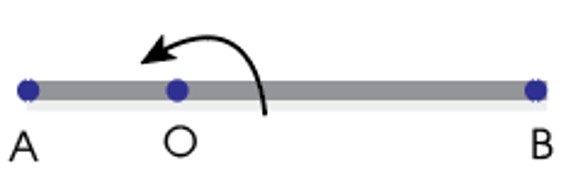
\includegraphics[scale=0.4]{../figs/D10-CK2-003-3}}
	\loigiai{
		
	}
\end{ex}
\Closesolutionfile{ans}
\begin{center}
	\textbf{--- HẾT ---}
\end{center}